% v4 Methods 3.4: the estimator suite, written to the Methods completeness
% contract (SESSION_35.md section 4, MC-1/2/3/5/6/7; provenance for every
% constant in outputs/session35/mc_provenance.md). Gupta, Chen & Wan
% (J. Fluid Mech. 1036, A24, 2026) is the completeness benchmark: state and
% observation model as numbered equations, every filter as update equations
% with every parameter, per-experiment parameters in one table.

\subsection{Estimating the state from the wall}
\label{sec:methods_estimators}
\label{sec:methods_estimator}

% Split out of the combined framework float (S3-C1) and moved here, next to the
% subsection that uses it, so the placer has a single-panel object and the
% caption describes one thing.
\begin{figure}
  \centering
  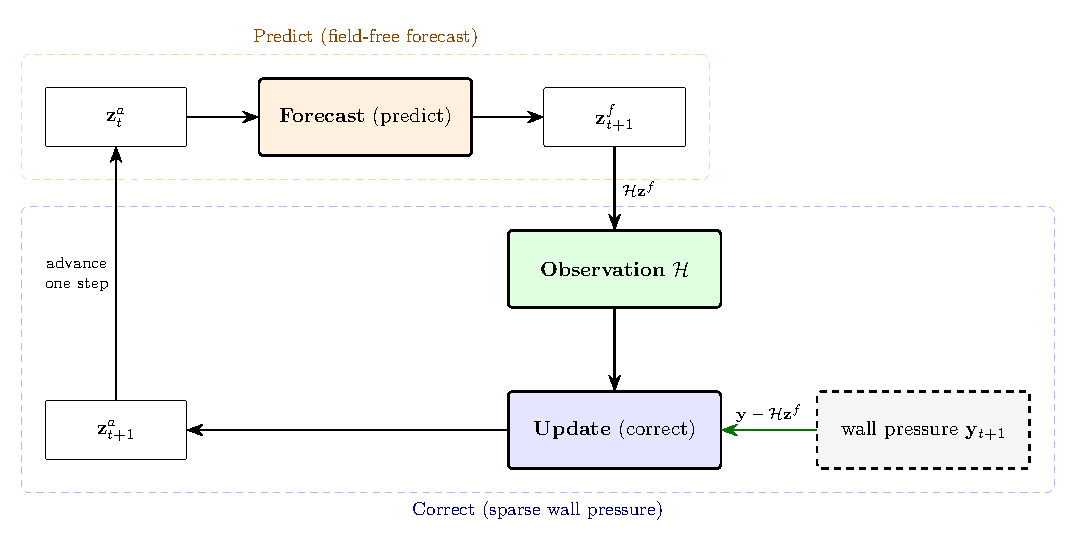
\includegraphics[width=\linewidth]{sections/figures/tikz/fig_estimation_loop.pdf}
  \caption{\rb{K}{S34-C1}{The deployment loop on its own, with the two slots that distinguish the four estimator configurations. The leakage guarantee sits here because the innovation path is what carries it.}The predict-correct loop at deployment, and the
  only route by which information reaches the state once the vorticity field is
  gone. \emph{Predict.} An ensemble of $\FilterMembers$ members, each a copy of
  the $\LatentDim$-dimensional coefficient state carrying its own perturbation,
  is advanced one frame through the prediction model without any field input;
  the forecast $\zvec^{f}_{t+1}$ is the result before any measurement is used.
  \emph{Correct.} The observation model maps that forecast to the observation it
  implies, $\hat{\mathbf{y}}_{t+1} = \mathcal{H}\zvec^{f}_{t+1}$; the wall
  pressure is then measured at $\FilterTaps$ span-averaged sensors, held out
  from training and placed by the per-model selection of
  appendix~\ref{app:osp}; and the innovation is the measurement minus that
  prediction. Only the innovation, never the measurement itself, moves the
  state. The subtraction is performed in sensor space for the base filter of
  \S\ref{sec:methods_enkf}, so $\mathcal{H}$ is the pressure read-out, and in
  encoded latent space for the filters of \S\ref{sec:methods_lae} and
  \S\ref{sec:methods_rexenkf}, where the sensor history is first lifted to a
  state estimate by $E_{\mathrm{obs}}$ and $\mathcal{H}$ is the identity. The
  update is a stochastic ensemble Kalman step: the innovation is multiplied by a
  gain built from the ensemble spread and the calibrated process and observation
  covariances $Q$ and $R$, and added to every member, giving the analysis
  $\zvec^{a}_{t+1}$ that the next predict step advances. All four estimator
  configurations are this one loop with only the two annotated slots swapped,
  the propagation $(F, Q)$ and the observation path. The production
  configuration is the two-stage one: the direct forecaster with the encoded
  observation inside the impact window, the matched transformer with the
  pressure sensors outside it. Table~\ref{tab:enkf} gives the settings per
  configuration, including the ensemble inflation applied before each update. No vorticity field enters at
  any point, the state is the same $\LatentDim$-vector at every step, and the
  frozen lift and wake probes are excluded from the innovation, which is what
  makes the reported analysis closure an estimate rather than a quantity the
  filter was handed.\re}
  \label{fig:estimation_loop}
\end{figure}

\rb{K}{S34-01}{Why estimation must be sequential, and the delay-embedding principle honestly scoped as an organising idea rather than a guarantee. \S4.5 is read against it.}At deployment the vorticity field is unavailable, and the wall pressure at a
single instant does not determine the state: one pressure frame recovers
little of the wake through any of the latents (\S\ref{sec:res_wall}). The
limitation is dynamical rather than instrumental, and it is relieved by
observing over a window of time rather than by adding sensors. The encounter
evolves on an attractor of low effective dimension, a limit cycle carrying a
gust excursion and a relaxation, into which the encoded latent concentrates its
variance (\S\ref{sec:res_latent_physics}). For such a system, delay-embedding
theory \citep{takens1981,sauer1991} establishes that a generic observation
function sampled over a window of delays reconstructs the attractor up to a
diffeomorphism, provided the product of the sensor count $K$ and the delay
count $m$ exceeds twice the attractor dimension. Reconstruction up to a
diffeomorphism means that the delay vector and the true state are related by a
smooth, smoothly invertible change of coordinates: the reconstruction preserves
the dynamics and every quantity that is a smooth function of the state, but it
does not return that state in its original coordinates, so a learned map from
the delay vector to $\zvec$ remains necessary. The genericity assumptions of
the theorem are not established for the finite, parametrically forced transient
family considered here, so we treat the result as an organising principle and
take the sensor-delay map of \S\ref{sec:res_wall} as the governing empirical
evidence. That map establishes two properties. A small number of sensors read
over a short window suffices, and lengthening the window compensates for
reducing the sensor count, so temporal resolution is exchangeable for spatial
resolution. The wake circulation, a coordinate to which the instantaneous
pressure is insensitive, is nonetheless recovered from the window, because the
circulation is dynamically coupled to the near-surface flow that the sensors do
resolve and therefore leaves a signature in the pressure history. Estimation
must accordingly be sequential, accumulating pressure innovations through
learned dynamics, which is the setting of data assimilation.\re

\rb{K}{S34-02}{The shared state-space problem, equations (5) and (6), plus the leakage guarantee. Every filter in the suite is defined by naming four ingredients of this pair.}Every estimator in this paper solves the same discrete state-estimation
problem on the frozen coefficient state. Write $\zvec_t \in \mathbb{R}^{d}$ for
the encoded state at frame $t$ and $\mathbf{p}_t \in \mathbb{R}^{K}$ for the
wall pressure at the $K$ selected sensors, with successive frames separated by
$\Delta t = \DtTc\,c/u_\infty$, the interval at which the cache stores the
simulation. The pair
\begin{equation}
  \zvec^{f}_{t+1} = F\!\left(\zvec^{a}_{t}\right) + \boldsymbol{\eta}_t,
  \qquad \boldsymbol{\eta}_t \sim \mathcal{N}(0, Q_t),
  \label{eq:ssm_dyn}
\end{equation}
\begin{equation}
  \mathbf{y}_t = h\!\left(\zvec_t\right) + \boldsymbol{\epsilon}_t,
  \qquad \boldsymbol{\epsilon}_t \sim \mathcal{N}(0, R),
  \label{eq:ssm_obs}
\end{equation}
defines each member of the suite once its four ingredients $(F, h, Q_t, R)$
are named; the remainder of this subsection does exactly that, and
table~\ref{tab:filter_params} collects every parameter. The superscripts
distinguish the two states of the assimilation cycle: $\zvec^{f}$ is the
forecast, obtained by advancing the previous estimate through $F$ before the
new measurement is used, and $\zvec^{a}$ is the analysis, the same state after
that measurement has corrected it. The frozen probes that read the lift and the
wake enstrophy from the state are excluded from the innovation by construction,
so the only measured quantity entering an update is the wall pressure and the
analysis closure reported in \S\ref{sec:res_da} is an estimate rather than a
quantity supplied to the filter (figure~\ref{fig:estimation_loop}).\re

\rb{K}{S34-03}{The two assimilation protocols, split out of S34-02 so the state-space definition and the evaluation setting are separate paragraphs. Every result states which protocol it follows.}Two assimilation protocols are used, and each result states which one it
follows. Under the envelope protocol, assimilation begins $\AssimPre$ frames
before impact and ends $\AssimPost$ frames after it, and the ensemble is
initialised at the start of that window without any field information. Under
the ladder protocol, assimilation runs over the whole encounter: the ensemble
is initialised at $t_0 = 9$, the first frame at which the ten-frame delay
window is complete, from the encoded observation there, and scoring is
restricted to the same impact window as the envelope protocol so that the two
are comparable. Every estimator in either protocol is fitted on the training
split alone. Each family senses at its own sensors, selected greedily on the
training split so as to best expose that family's own state, with a shared
target-blind array used wherever a sensor-budget claim must not depend on a
placement tuned to any one model; the selection criterion and the two arrays are
given in appendix~\ref{app:osp}.\re

\subsubsection{Base stochastic ensemble filter}
\label{sec:methods_enkf}

\rb{K}{S34-04}{The base filter and its fitted ingredients, including the encounter-grouped split behind $R$. It is the reference configuration, not the production estimator.}The base filter is a stochastic ensemble Kalman filter in the
perturbed-observation form of \citet{burgers1998}, following
\citet{evensen2003}, with $N = \FilterMembers$ members. It is the reference
configuration against which the others are read, not the production estimator
of \S\ref{sec:methods_rexenkf}, but its update is the one every configuration
in the suite uses. The prediction model $F$ is the matched autoregressive
transformer of \S\ref{sec:methods_arch}, refitted on the frozen pooled training
trajectories; each member carries its own buffer of past analysis states (at
most $32$ frames) and is advanced one step per frame. The process noise is
state-independent, $Q_t \equiv Q$, estimated as the sample covariance of
one-step teacher-forced predictor residuals over $256$ training
sub-trajectories of length $32$, with a $10^{-6}$ diagonal floor. The
observation map $h$ is a ridge-regularised linear read-out from the state to
the $K$ sensors. It is fitted on four fifths of the training encounters and the
observation-noise covariance $R$ is the diagonal residual variance of that map
on the remaining fifth, with floor $10^{-6}$. The split is by whole encounter
rather than by frame: frames within one encounter are strongly autocorrelated,
so a frame-wise split would place near-copies of the fitted data in the
held-out set and return an $R$ far smaller than the error the filter actually
meets, which is the one quantity that tells the filter how much to trust its
sensors. Both parts of the split lie inside the training split, so no held-out
encounter is touched.\re

\rb{K}{S34-05}{The ensemble-Kalman gain and update, written in the cross-covariance form the code implements, with the plain-language reading of what the gain does.}Write $\bar{\zvec}^{f}_t = N^{-1}\sum_i \zvec^{f,(i)}_t$ for the ensemble mean
of the forecast, $X^{f}_t = [\zvec^{f,(i)}_t - \bar{\zvec}^{f}_t]_i$ for the
$d \times N$ matrix of member deviations from it, and
$Y^{f}_t = [h(\zvec^{f,(i)}_t) - \overline{h(\zvec^{f}_t)}]_i$ for the same
deviations carried through the observation map. The gain and the update are
\begin{equation}
  \Sigma^{zy}_t = \frac{X^{f}_t (Y^{f}_t)^{\mathsf{T}}}{N - 1}, \qquad
  \Sigma^{yy}_t = \frac{Y^{f}_t (Y^{f}_t)^{\mathsf{T}}}{N - 1} + R, \qquad
  K_t = \Sigma^{zy}_t \left(\Sigma^{yy}_t\right)^{-1},
  \label{eq:enkf_gain}
\end{equation}
\begin{equation}
  \zvec^{a,(i)}_t = \zvec^{f,(i)}_t
  + K_t \left(\mathbf{y}_t + \boldsymbol{\epsilon}^{(i)}_t
  - h\!\left(\zvec^{f,(i)}_t\right)\right),
  \qquad \boldsymbol{\epsilon}^{(i)}_t \sim \mathcal{N}(0, R).
  \label{eq:enkf_update}
\end{equation}
where $\Sigma^{zy}$ measures how each coordinate of the state co-varies
with each sensor across the ensemble, and $\Sigma^{yy}$ is how much the
predicted observation varies, from the spread of the ensemble and from sensor
noise together. Their ratio $K_t$ is the weight given to being wrong at the
wall, so a state coordinate that the sensors see clearly is corrected hard and
one they barely see is left near its forecast. Each member is then moved by its
own innovation, computed against its own independently perturbed copy of the
measurement; perturbing the measurement per member is what stops the ensemble
from collapsing to zero spread as it is corrected, and it is what makes the
filter stochastic. Written this way the gain is formed from ensemble
cross-covariances, exactly as implemented, and no $d \times d$ forecast
covariance is ever built; for the linear $h$ used here this is algebraically
the textbook $P^{f}H^{\mathsf{T}}(HP^{f}H^{\mathsf{T}} + R)^{-1}$.\re

\rb{K}{S34-06}{Multiplicative inflation, what it corrects, and the field-free initialisation. Small but load-bearing: the inflation values differ by family.}Multiplicative inflation $\zvec^{f,(i)} \leftarrow \bar{\zvec}^{f} +
\rho\,(\zvec^{f,(i)} - \bar{\zvec}^{f})$ is applied before the update. It
rescales the ensemble about its mean, widening the spread when $\rho > 1$; the
standard remedy for the tendency of a small ensemble to become overconfident,
which if left alone makes $\Sigma^{yy}$ too small, the gain too large and the
filter progressively deaf to its sensors. Here $\rho$ is selected per family on
the validation split only ($\rho = \FeRhoJepa$ for the predictive and linear
families, $\rho = \FeRhoFukami$ for the reconstructive one). The ensemble is
initialised at the window start from a windowed pressure-to-state regressor (a
Nystr\"om radial-basis ridge with $300$ components on a $12$-frame causal
pressure window) by sampling its training-residual covariance around the
regressed mean, so no field information enters the filter at any time. The
frozen observable probes that score the filter never enter the innovation: the
only measured quantity in \eqref{eq:enkf_update} is the $K$-sensor wall
pressure.\re

\subsubsection{The \LinLatKF{} with encoded observations}
\label{sec:methods_lae}

\rb{K}{S34-07}{Carries equation (9), the encoded observation used by three of the four configurations, and the one fixed definition of consistency failure. Load-bearing well beyond its own subsection.}This configuration replaces both ingredients of the base filter with their
simplest stable counterparts, and it exists to separate what the estimator
contributes from what the learned dynamics contribute: if a linear propagation
driven by a full-state observation matches a nonlinear one, the gain was in the
sensing rather than in the model. It follows the latent-space assimilation
construction of \citet{tong2026}. The dynamics are linear, $F(\zvec) = A\zvec$,
with $A$ the ridge solution of $\zvec_{t+1} \approx A \zvec_t$ over all training
transitions, followed by a projection of its singular values onto $[0, 1]$. That
projection is what keeps the propagation stable: a singular value above one is a
direction the operator amplifies at every step, so a long rollout diverges along
it, and clipping the spectrum removes those directions outright rather than
penalising them as \citet{tong2026} do. $Q$ is the covariance of the resulting
fit residuals. The observation side replaces the sparse sensors by an encoded
full-state observation: a delay-embedding operator lifts the normalised sensor
history $\mathbf{p}_{t-m+1:t} \in \mathbb{R}^{Km}$ with $m = 10$ (causal,
edge-padded), and a ridge map $W$ regresses it onto the state, so that
\begin{equation}
  \mathbf{y}_t = E_{\mathrm{obs}}\!\left(\mathbf{p}_{t-m+1:t}\right)
  = W^{\mathsf{T}} \operatorname{vec}\!\left(\mathbf{p}_{t-m+1:t}\right),
  \qquad h = \mathrm{Id}, \qquad
  R = \Gamma,
  \label{eq:eobs}
\end{equation}
with $\Gamma$ the covariance of the $E_{\mathrm{obs}}$ training residuals
plus a $10^{-8}$ jitter. The same $E_{\mathrm{obs}}$, evaluated framewise
with no dynamics at all, is the \StaticInv{} that anchors the estimator
ladder. Filter consistency failure is declared by one fixed criterion everywhere
in the paper: the normalised innovation squared exceeds the $\chi^2_{0.99}$
quantile at the observation dimension for five or more consecutive frames, or
any analysis Mahalanobis ratio exceeds $3$. Both tests ask whether the filter's
own error bars are honest, that is whether the innovations are as large as the
ensemble spread and $R$ together say they should be; persistently larger means
the ensemble has become overconfident and the gain is too small for the error it
faces. It is therefore distinct from a large-error encounter, for which the
analysis lift itself fails (impact-phase $R^2$ below $-1$), and a filter can
post consistency failures while its mean still tracks the load.\re

\subsubsection{Forecast-derived state-dependent process noise}
\label{sec:methods_rexenkf}

\rb{K}{S34-08}{The production route: state-dependent noise, its two independent calibrations, and the two-stage schedule. This is the estimator the headline number comes from.}The \FnoiseKF{} keeps the encoded observation \eqref{eq:eobs} and
replaces the member propagation by the \DirectFC{} of
\S\ref{sec:methods_rex}: each member is advanced by the one-step median
forecast, and the process noise is read off the forecaster's own
uncertainty band at forecast time,
\begin{equation}
  \zvec^{f,(i)}_{t+1} = \hat{\zvec}^{\,q_{0.5}}_{t+1}
  + c\,\boldsymbol{\sigma}_{t+1} \odot \boldsymbol{\xi}^{(i)},
  \qquad
  \boldsymbol{\sigma}_{t+1}
  = \frac{\hat{\zvec}^{\,q_{0.9}}_{t+1} - \hat{\zvec}^{\,q_{0.1}}_{t+1}}
         {2 \times 1.28155},
  \qquad \boldsymbol{\xi}^{(i)} \sim \mathcal{N}(0, \mathrm{Id}),
  \label{eq:rex_q}
\end{equation}
where $\hat{\zvec}^{\,q}$ is the forecaster's predicted $q$th quantile of the
next state, $\odot$ is the elementwise product, and $\boldsymbol{\xi}^{(i)}$ is
an independent standard normal draw per member. In words: every member is put at
the forecaster's median prediction and then scattered about it by an amount the
forecaster itself nominates, so the ensemble is wide exactly where the
forecaster expects to be wrong. The divisor turns a quantile band into a
standard deviation: for a Gaussian the interval from $q_{0.1}$ to $q_{0.9}$ is
$2\,\Phi^{-1}(0.9) = 2 \times 1.28155$ standard deviations wide, with $\Phi$ the
standard normal distribution function, so dividing the predicted band by that
number reads off the equivalent $\boldsymbol{\sigma}$. The process noise
$Q_t = c^2\operatorname{diag}(\boldsymbol{\sigma}_{t+1})^2$ is therefore
state-dependent: unlike the fixed $Q$ of the base filter, it grows and shrinks
with the difficulty of the step, which is the property the whole configuration
exists to exploit.\re

\rb{K}{S34-09}{The two independent calibrations of the band scale and the NIS statistic they are judged by. Which calibration wins is itself a result.}The single scalar $c$ is the filter's only tuned quantity and it carries two
independent calibrations, both on validation data alone. The production value
$c = 1.77$ is the coverage calibration: it is the scale at which the one-step
$q_{0.1}$ to $q_{0.9}$ band actually contains $80\,\%$ of held-out training
transitions, as an $80\,\%$ band should. The second calibration, fixed in
advance of seeing any value, tunes $c$ for filter consistency instead. It asks
whether the innovations are the size the filter claims to expect, measured by
the normalised innovation squared
\begin{equation}
  \mathrm{NIS}_t = \frac{1}{d}\,\nu_t^{\mathsf{T}} S_t^{-1} \nu_t,
  \qquad \nu_t = \mathbf{y}_t - \bar{\zvec}^{f}_t,
  \qquad S_t = P^{f}_t + \Gamma,
  \label{eq:nis}
\end{equation}
in which $\nu_t$ is the innovation and $S_t$ is the covariance the filter
predicts for it, the ensemble spread $P^{f}_t$ plus the observation noise
$\Gamma$. Dividing by the observation dimension $d$ makes the expected value one
when the filter's uncertainty is honest: below one it is overdispersed, claiming
more uncertainty than it has, and above one it is overconfident. We select $c$
by driving the pooled impact-phase $\mathrm{NIS}$ toward one over the fixed grid
$c \in \{1.0, 1.4, 1.77, 2.5, 3.5, 4.5, 6.0\}$, on the held-out encounters of
the training cases, followed by a single frozen run on the test splits. The two
calibrations need not agree, and which one wins is itself a result
(\S\ref{sec:res_da}). The \TwoStageKF{} applies the
encoded-observation update \eqref{eq:eobs} with the median-forecast propagation
\eqref{eq:rex_q} inside the impact window only, and outside it propagates
members with the matched transformer and assimilates in sensor space through
the linear map of \S\ref{sec:methods_enkf}; the schedule boundary is the
frozen impact-window mask of the cache and is not tuned. One further member of
the suite is a reanalysis rather than a filter: a fixed-lag
Rauch--Tung--Striebel smoother on the linear stack of \S\ref{sec:methods_lae},
which revises each estimate once five later frames of pressure have arrived and
so buys accuracy at a fixed reporting latency of $0.25\,c/u_\infty$. Its
recursion is given in appendix~\ref{app:rts}.\re

% S34-06 (the RTS recursion) moved to appendix C and S34-07 (the greedy
% placement criterion) to appendix B, on Carlos's 2026-08-13 comments. Both were
% already classed A in the relevance ledger. The brief forms stay here: the
% smoother in the sentence above, the placement in S34-02, because both are
% referred to from the Results and a reader needs to know they exist without
% needing their equations. The old labels went with the content; every call
% site now points at app:rts or app:osp.
